Le simulazioni sono state ottenute abilitando nel simulatore le componenti
corrispondenti alle seguenti flags:
\begin{lstlisting}[language=matlab,breaklines=true]
GravityTypeFlag=1;		%(1=J2 Gravity Model/=0 Spherical)
GravityGradientTorqueFlag=1;	%1=Gravity Gradient Torque ON/0=OFF 
DragForceDisturbancesFlag=1;	%0=Drag Force Disturbance OFF/1=OFF
DragTorquesDisturbancesFlag=1;	%0=Drag Torque Disturbance OFF/1=ON
DragFreeControlFlag=1;		%0=Drag Free Control OFF/1=ON
AttitudeControlFlag=1;		%0=Attitude Control OFF/1=ON
\end{lstlisting}

\begin{SCfigure}[0.7][ht]
	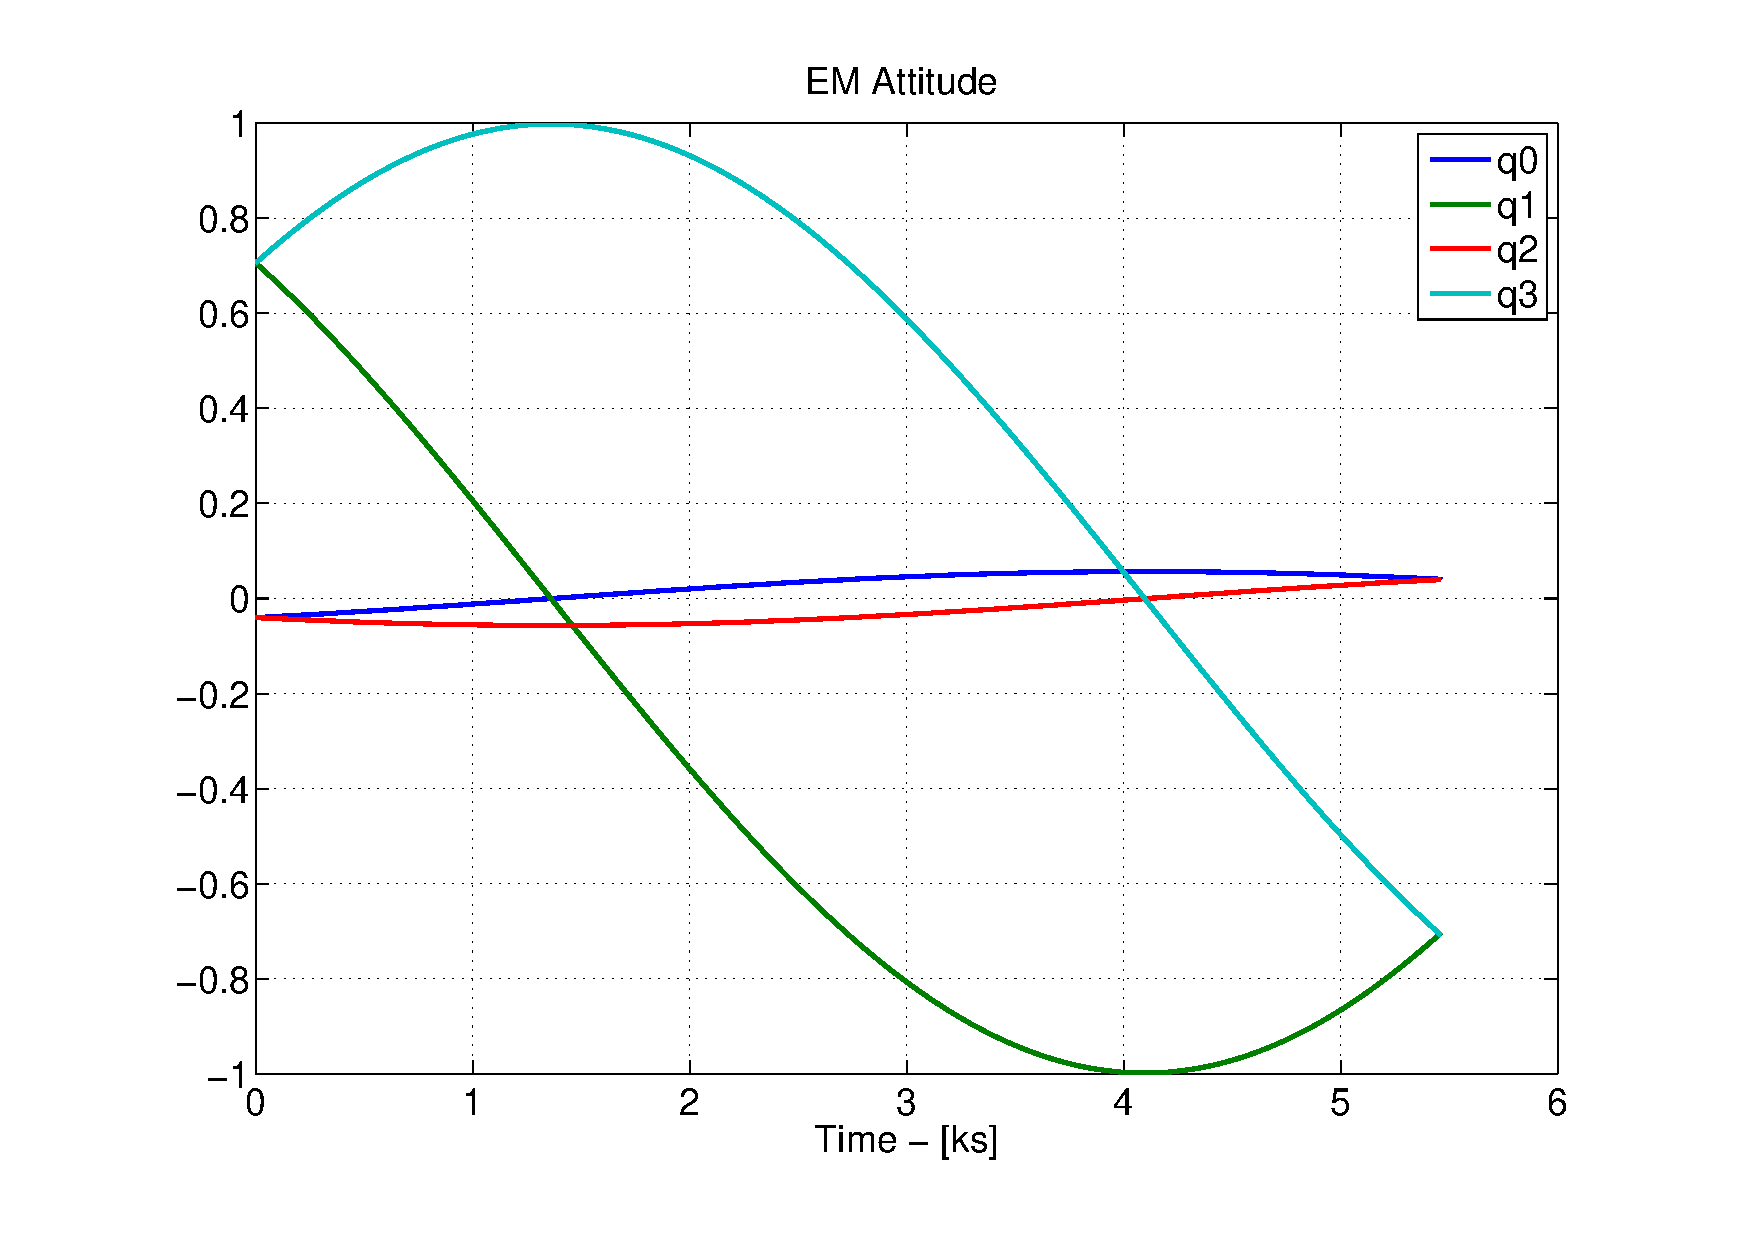
\includegraphics[width=.6\textwidth]{control/attitude_control/images/EmbeddedModelAttitude.pdf}
	\caption{\emph{Quaternione di assetto} --- Quaternione assetto stimato
	dall'embedded model a partire dallo star tracker}
	\label{fig:drag-acceleration}
\end{SCfigure}

\begin{SCfigure}[0.7][ht]
	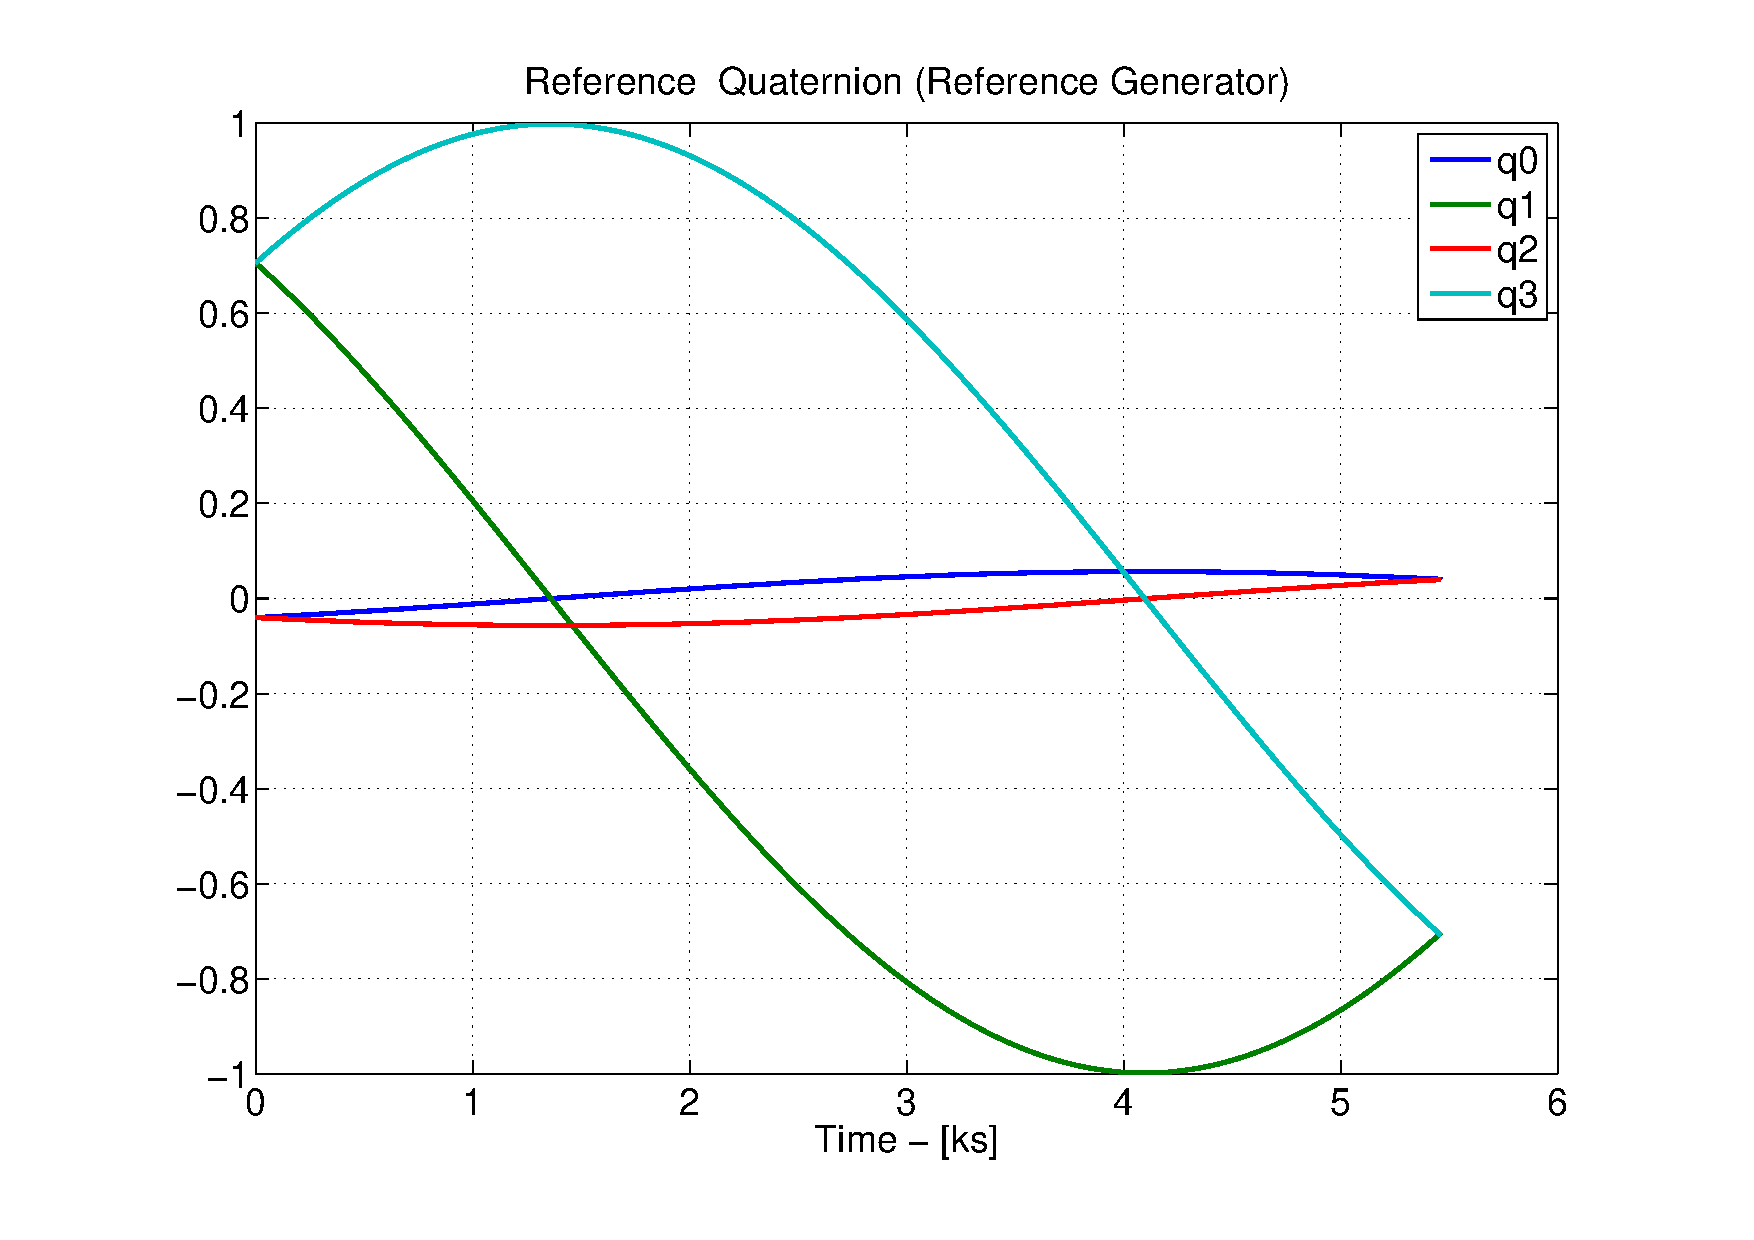
\includegraphics[width=.6\textwidth]{control/attitude_control/images/ReferenceQuaternion.pdf}
	\caption{\emph{Quaternione di riferimento} --- Quaternione rappresentante il
	riferimento LORF nel sistema di riferimento inerziale, deve essere inseguito
	dal controllo}
	\label{fig:drag-acceleration}
\end{SCfigure}

\begin{SCfigure}[0.7][ht]
	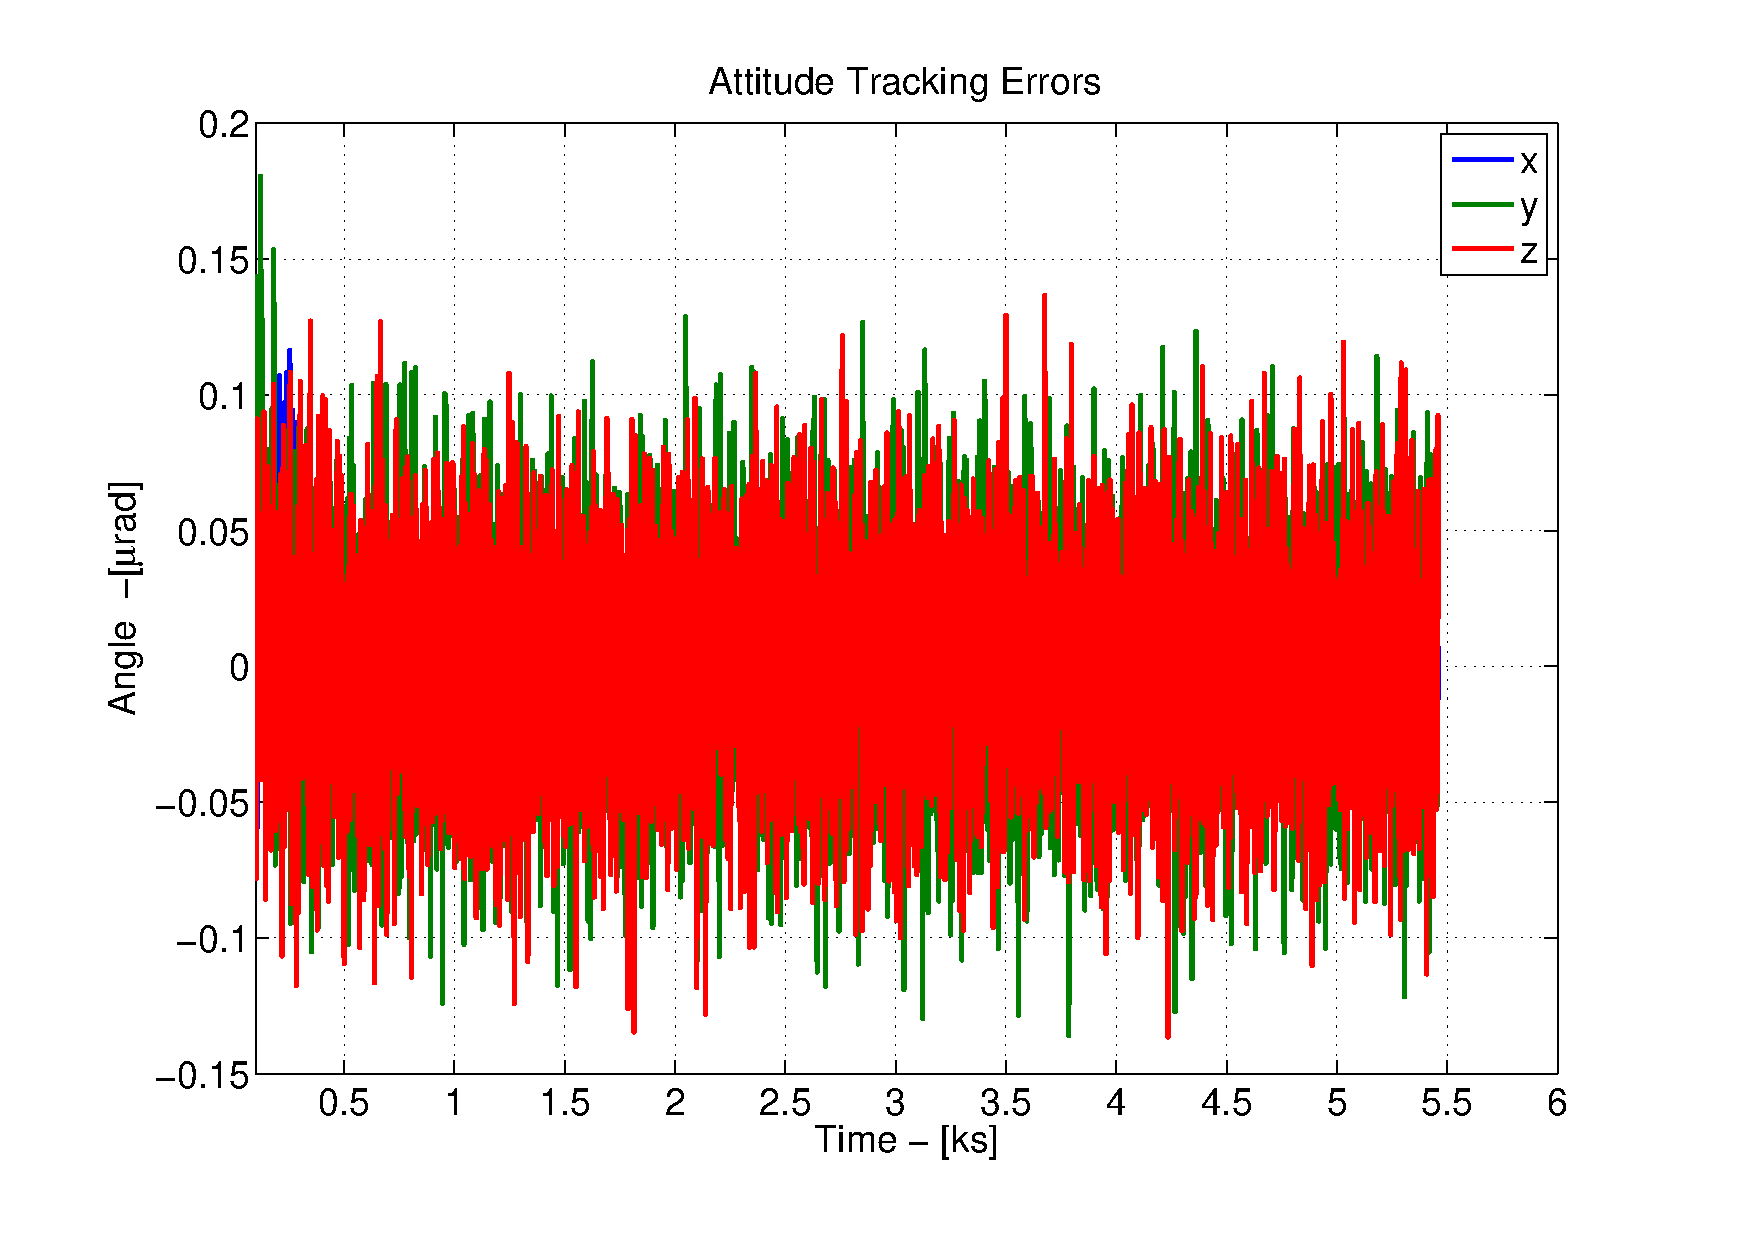
\includegraphics[width=.6\textwidth]{control/attitude_control/images/TrackingError.pdf}
	\caption{\emph{Errore di inseguimento} --- L'errore si mantiene nei requisiti
	di precisione richiesti}
	\label{fig:drag-acceleration}
\end{SCfigure}